In this section we will present the results of simulations and compare them with previous methods and true optima.

\subsection{Initial condition}
	First we have to check if changing the initial state makes any difference to the output of an algorithm. This is achieved via setting a different seed and repeating algorithms for the same number of iterations. Seeds guarantee us the different ``randomness'' with each seed. It is because the generators are only generating \textit{pseudo-random numbers} which we can control. Both algorithms will have the same seeds and in our case these are $1,2,3,4$. We use default parameters of temperature $\tau=2$ and cooling schedule $t_n=1$.
	\begin{figure}[!htb]
		\centering
		\begin{subfigure}{0.45\textwidth}
			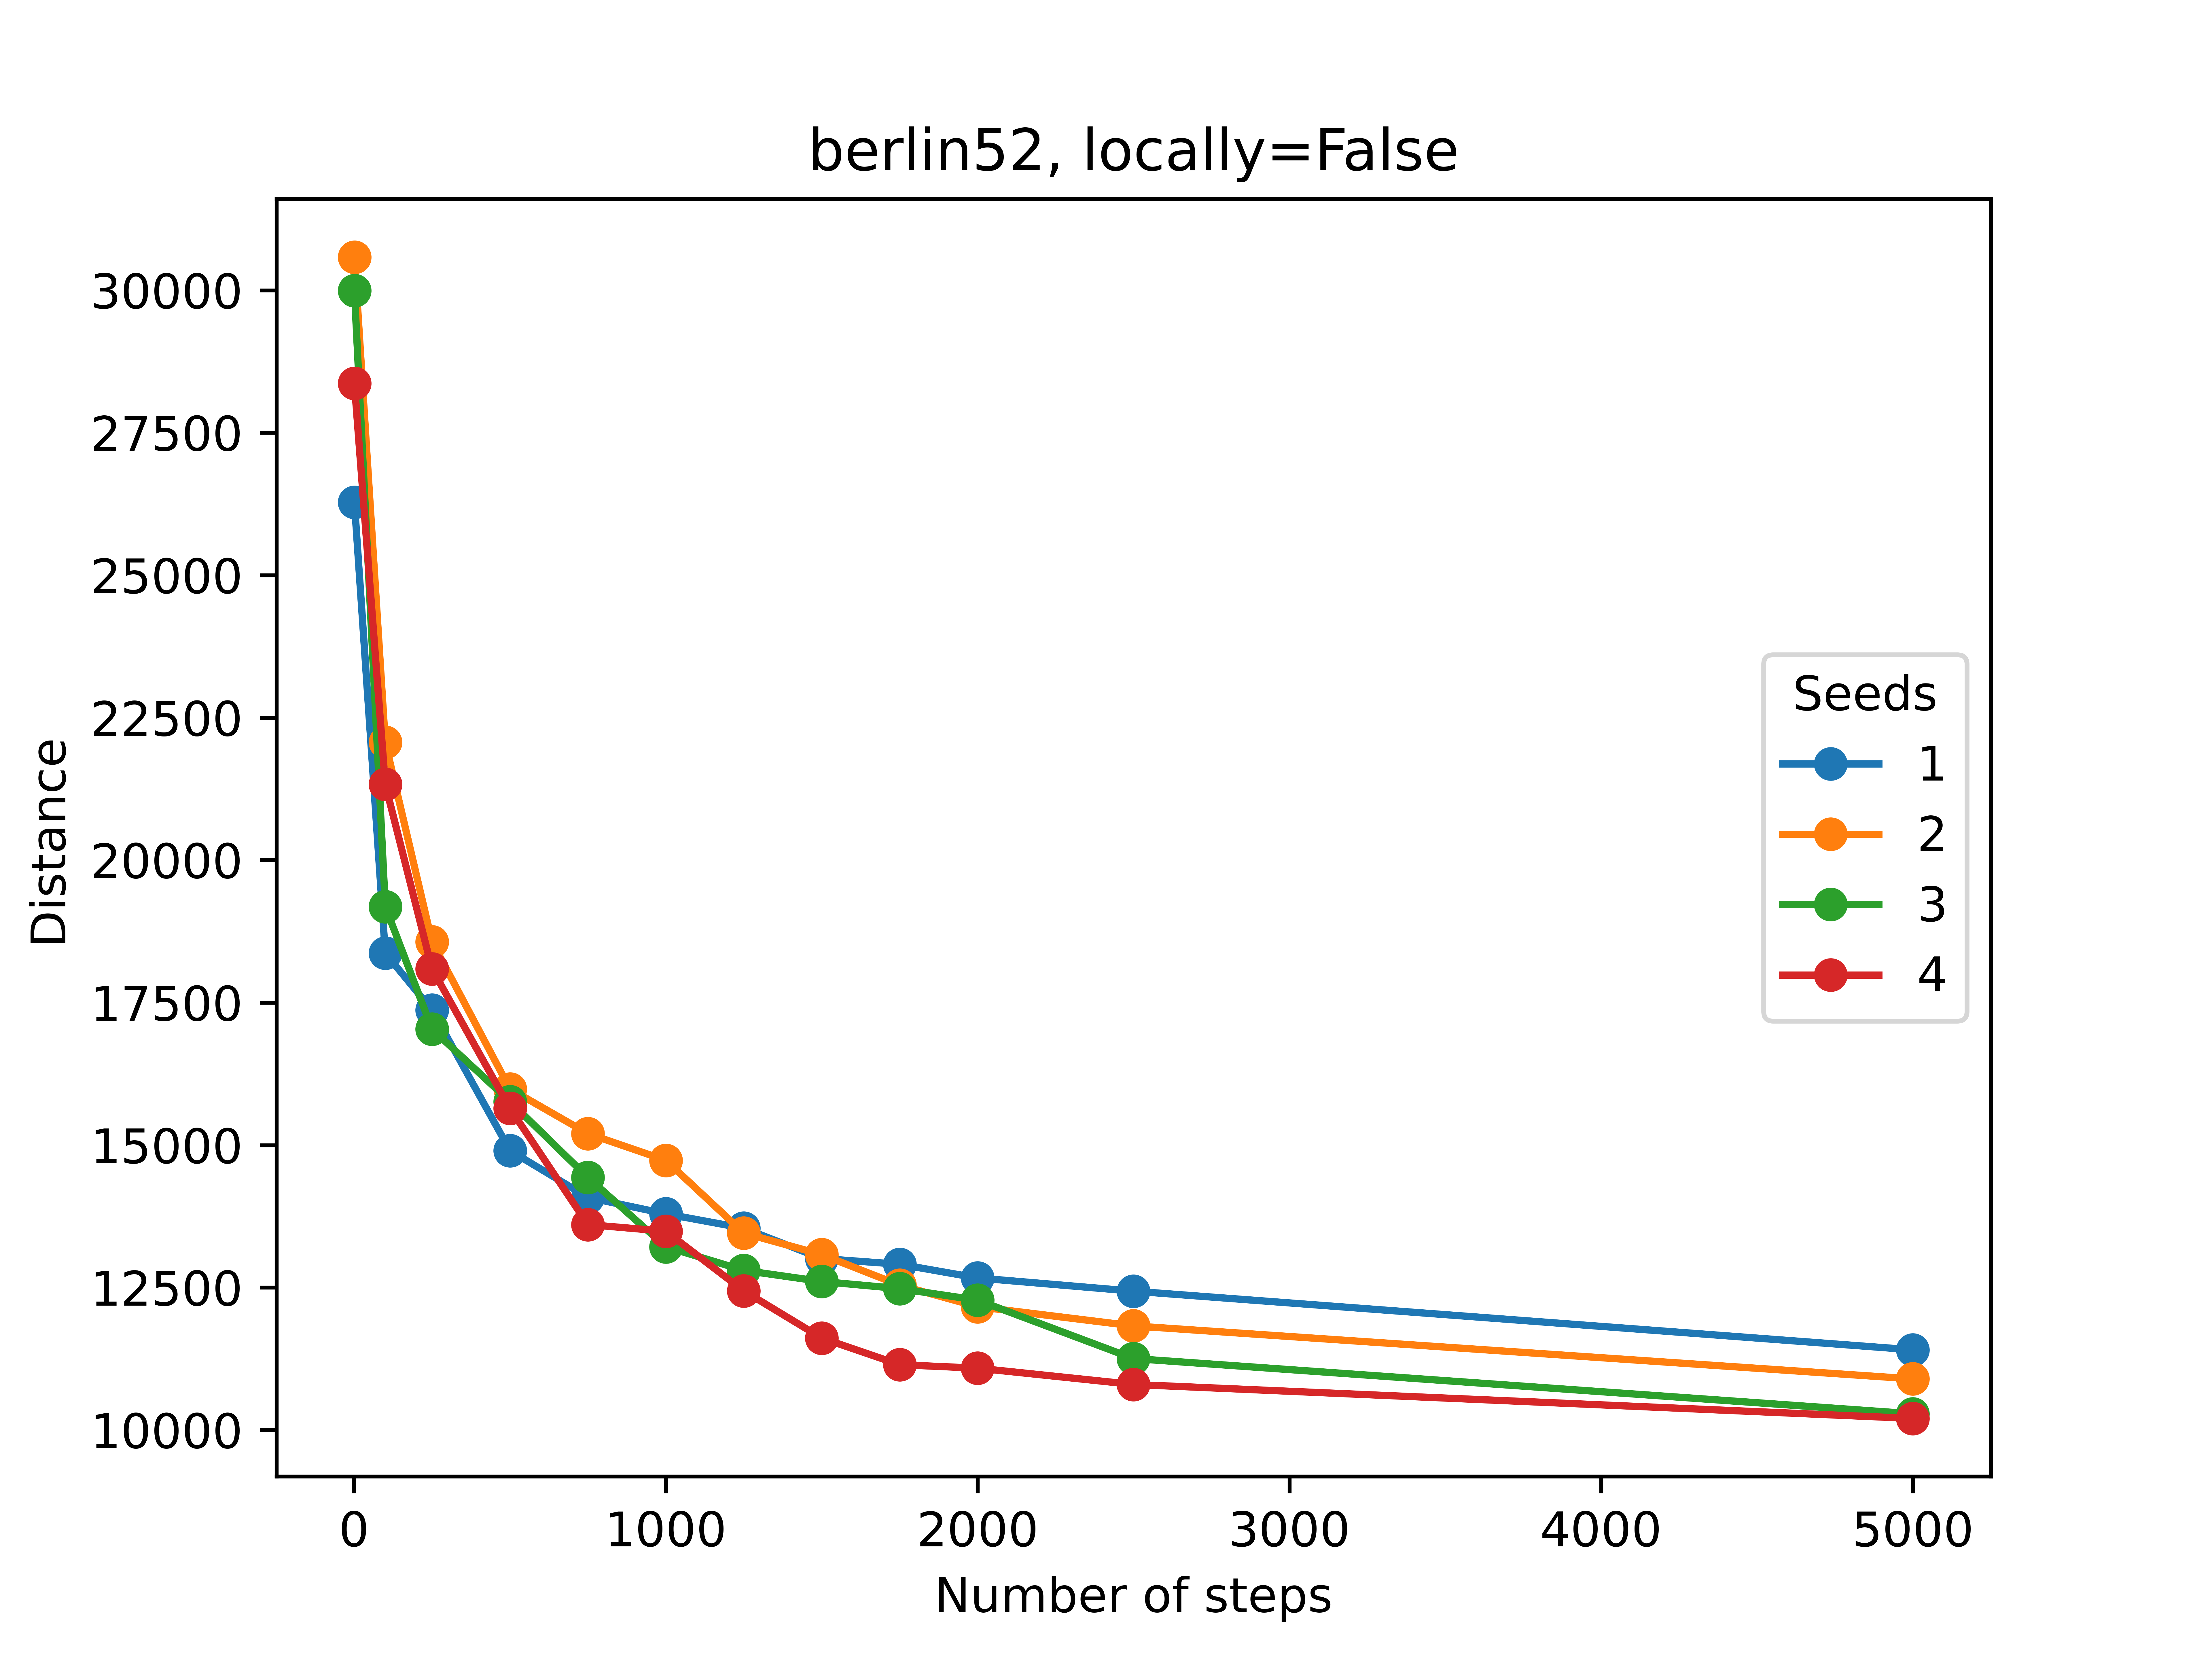
\includegraphics[width=\textwidth]{plots/berlin52_seeds_locally=False}
			\subcaption{Random candidates.}
		\end{subfigure}
		\begin{subfigure}{0.45\textwidth}
			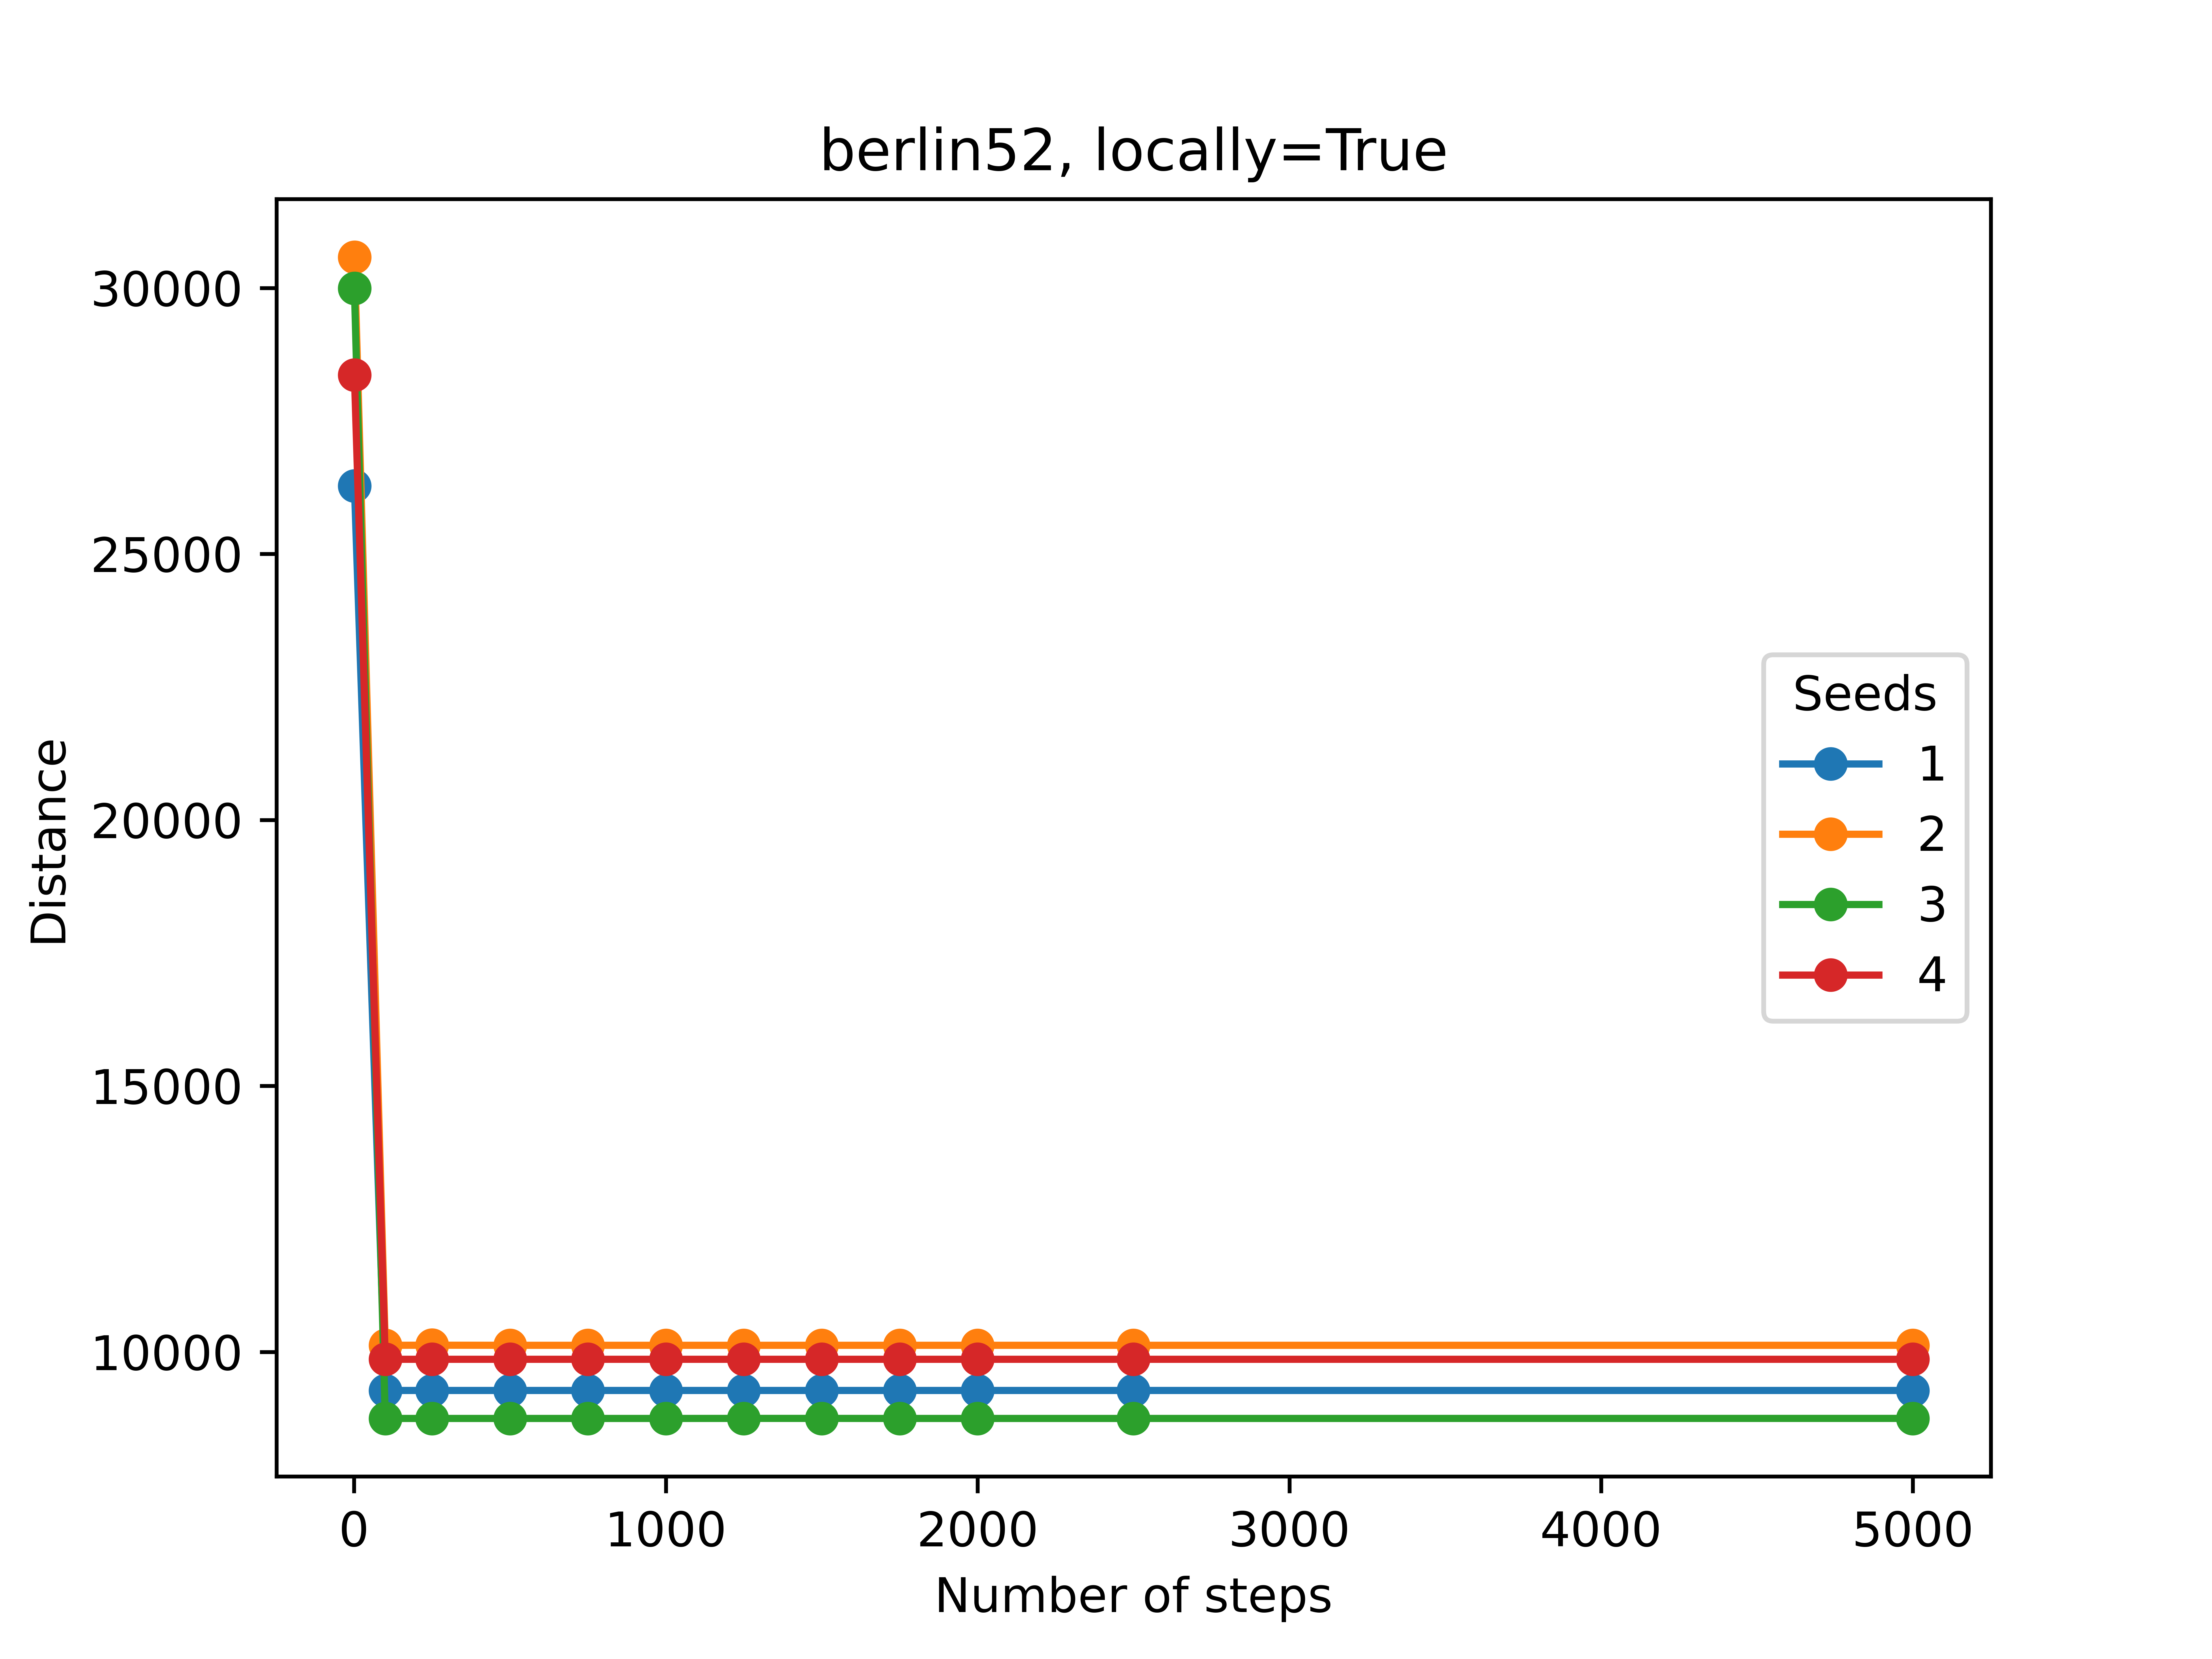
\includegraphics[width=\textwidth]{plots/berlin52_seeds_locally=True}
			\subcaption{Locally-informed proposals.}
		\end{subfigure}
		\caption{Distances over number of steps for \textit{berlin52} dataset.}
		\label{fig:berlin52_seeds}
	\end{figure}
	
	\begin{figure}[!htb]
		\centering
		\begin{subfigure}{0.45\textwidth}
			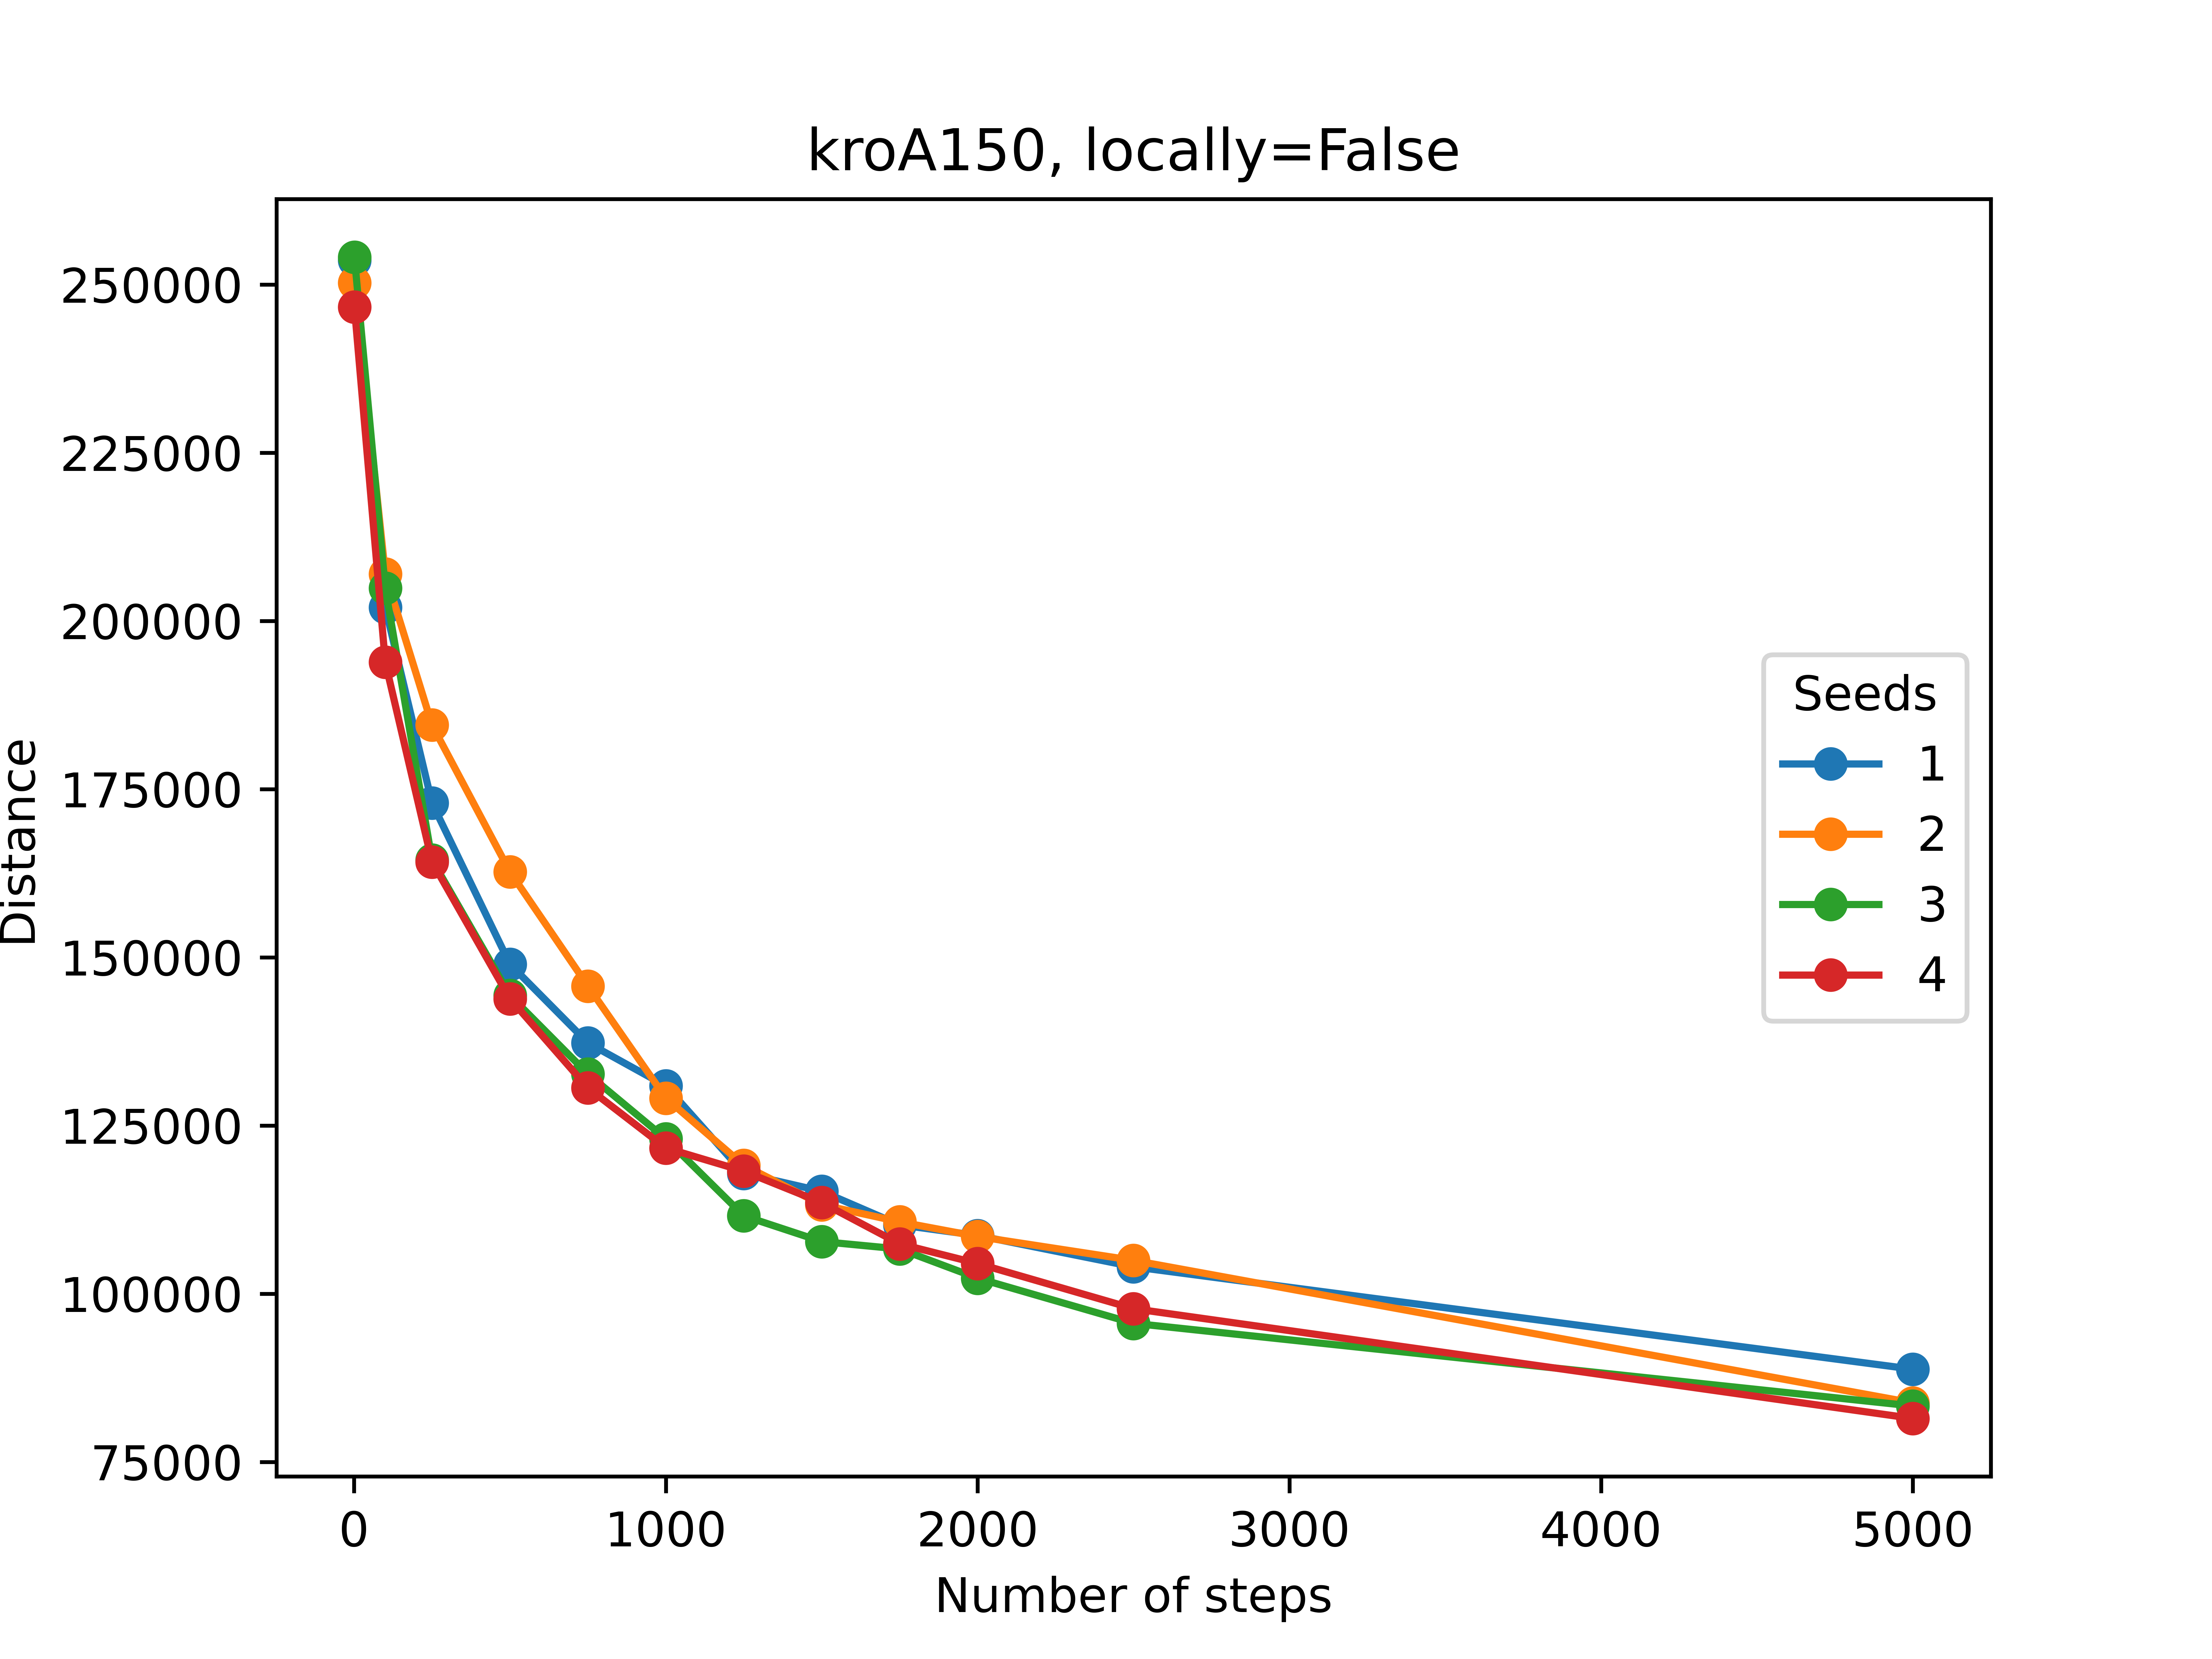
\includegraphics[width=\textwidth]{plots/kroA150_seeds_locally=False}
			\subcaption{Random candidates.}
		\end{subfigure}
		\begin{subfigure}{0.45\textwidth}
			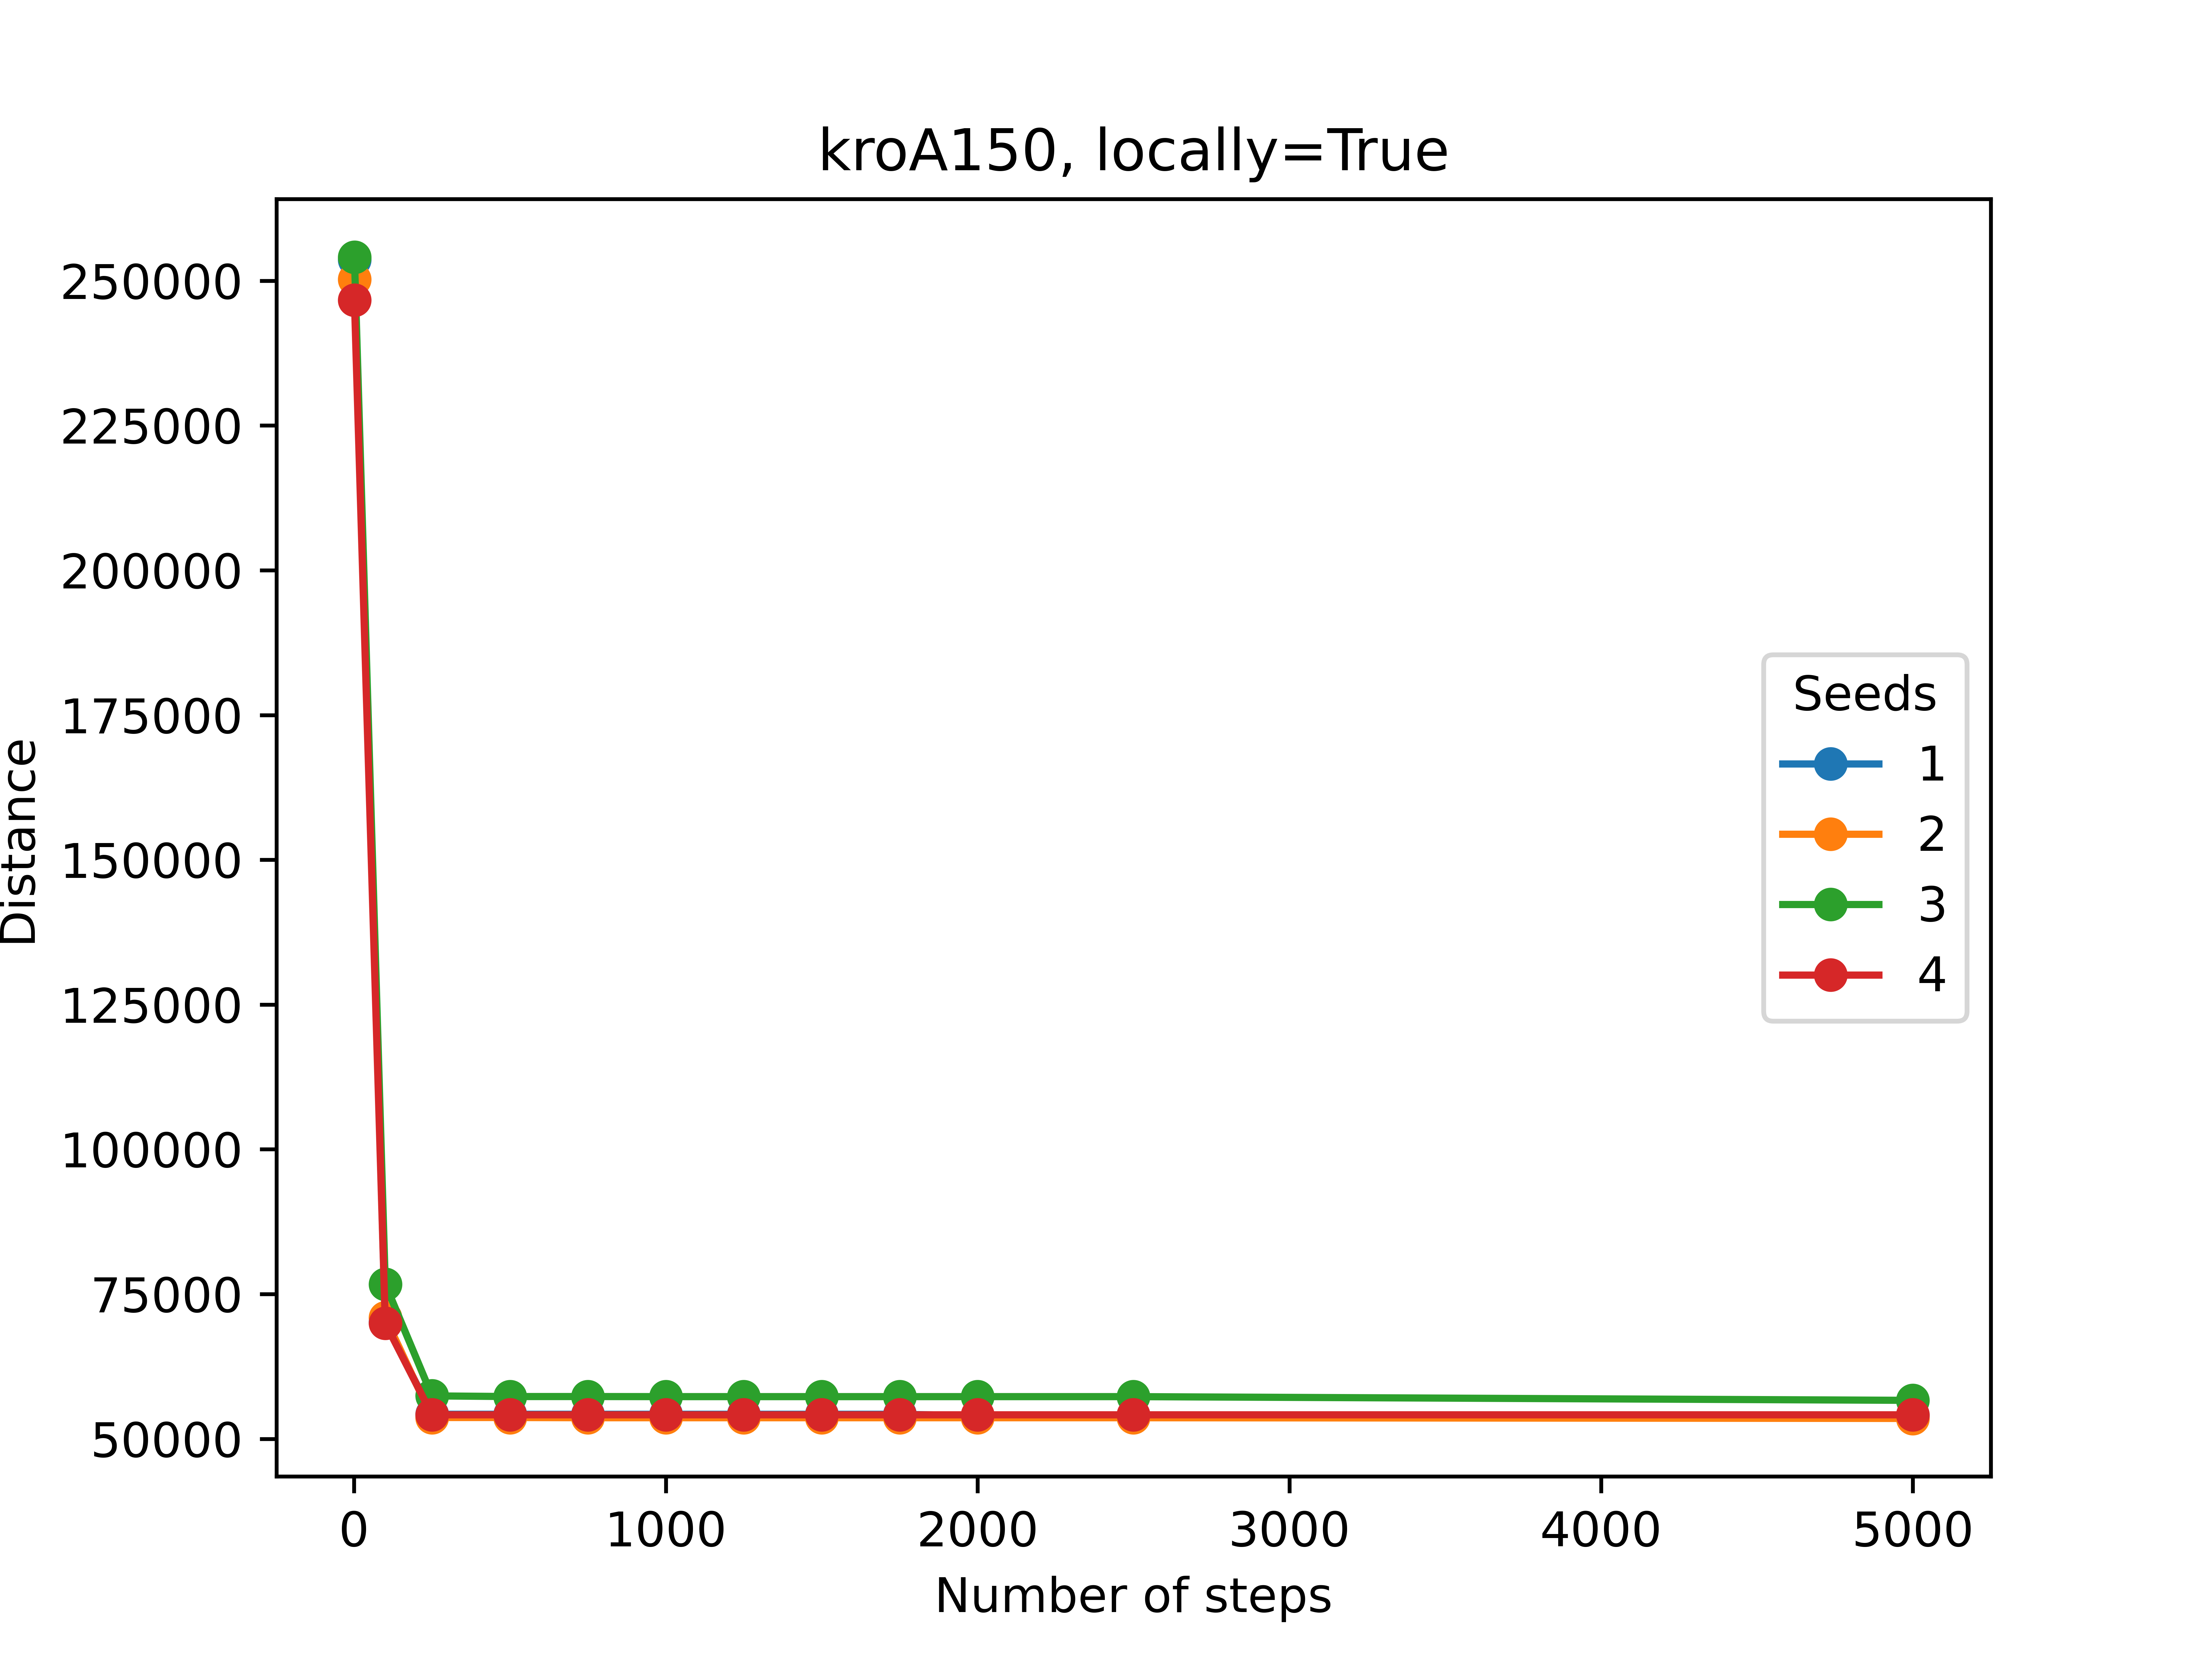
\includegraphics[width=\textwidth]{plots/kroA150_seeds_locally=True}
			\subcaption{Locally-informed proposals.}
		\end{subfigure}
		\caption{Distances over number of steps for \textit{kroA150} dataset.}
		\label{fig:kroA150_seeds}
	\end{figure}

	Both plots \ref{fig:berlin52_seeds} and \ref{fig:kroA150_seeds} suggest that initial state matters for finding a better tour, but it is not changing the behavior of algorithms.
	
\subsection{Simulated annealing}
	Before we proceed with comparing algorithms we need to find out if simulated annealing is improving them. We will compare parameters $t_n=1$ and $t_n= \frac{3}{\log(n+2)}$ where $n$ is a number of step. The temperature parameter for locally-informed proposals will stay at default $\tau=2$ and seed $1$.